\section{System Description}

\begin{figure}
  \centering
  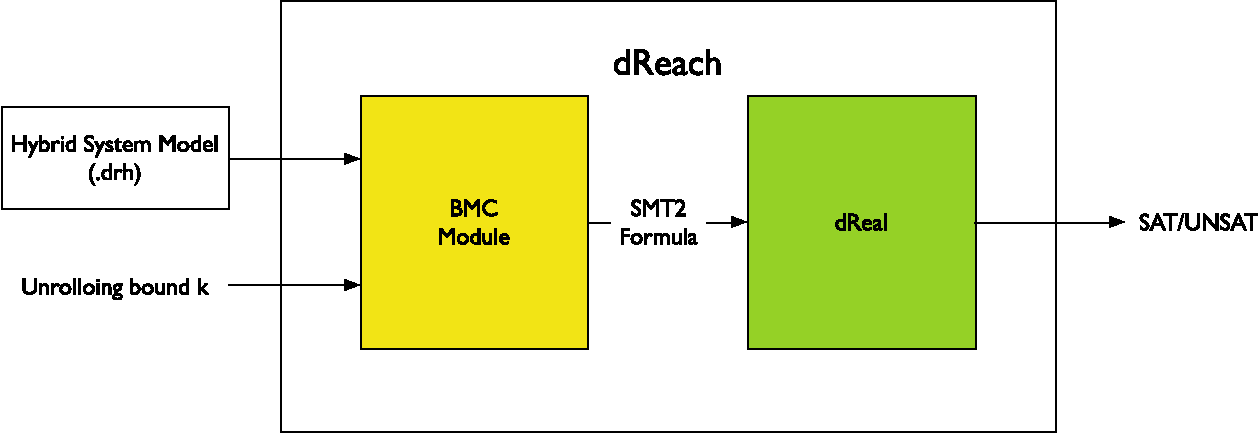
\includegraphics[width=\textwidth]{images/dReach}
  \caption{System Description of \dReach{}}
  \label{fig:system-description}
\end{figure}

Figure~\ref{fig:system-description} illustrates the architecture of
\dReach{}. We provide a domain-specific lanaguage to describe a hybrid
system and specify its safety properties. Given an input model,
specification, and unrolling bound $k$, \dReach{} reduces the
$\delta$-reachability problem to a $\delta$-decision problem of
formulas over the reals by providing a corresponding SMT encoding for
the problem. Then we answer the bounded reachability queries by using
our nonlinear SMT solver \dReal{}~\cite{DBLP:conf/cade/GaoKC13} to
solve the encoded problems.

\subsection{drh: a Language for Modeling and Specifying Hybrid Systems}

We define \texttt{drh}, a small language for describing hybrid systems
and specifying their initial and safety conditions. It consists of
five sections - macro definitions, variable declarations, mode
definitions, and initial condition, and goals.
\begin{align*}
  \textit{drh} := \ & \textit{macro-definition}^*\\
                  & \textit{variable-declaration}^+\\
                  & \textit{mode-definition}^+\\
                  & \textit{initial-condition}\\
                  & \textit{goal}^+
\end{align*}
In macro definitions, we allow users to define C-preprocessor macros
which can be used in following sections. Macros are expanded before
the other parts are processed.

A variable declaration has a form:
\[
\textit{variable-declaration} \ := \ \texttt{[}
                                     \textit{l}
                                     \texttt{,}
                                     \ \textit{u}
                                     \texttt{]}
                                     \ \textit{var}
                                     \texttt{;}
\]
and it declares a real variable $var$ whose domain is $[l, u] \in
\mathbb{IR}$. A special variable \textit{time} has to be delcared to
specify the time bound of bounded model checking.

A mode definition consists of mode id, mode invariant, flow, and jump.
\begin{align*}
  \textit{mode-definition} \ := & \ \texttt{\{}
                                    \texttt{mode} \ \textit{id}\texttt{;}\\
                           & \ \ \  \texttt{invt}:(\textit{formula} \texttt{;})^+\\
                           & \ \ \  \texttt{flow}:\textit{ode}^+\\
                           & \ \ \ \texttt{jump}:\textit{jump}^+ \texttt{\}}
\end{align*}
\textit{id} is a unique unsigned integer assigned to a mode. An
invariant is a conjuction of logic formulae which must hold in a mode.
A flow describes a continuous dynamics of a mode by providing a set of
ordinary differential equations (\textit{ode}s) which is a form of
``\texttt{d/dt[}\textit{x}\texttt{]=}\textit{exp}''. \textit{jump} is
a form of ``\textit{guard} \texttt{==>} \texttt{@}\textit{n}
\textit{reset}'' where \textit{guard} is a logic formula specifying a
condition to make a transition, $n$ is an id of target mode, and
\textit{reset} is a logic formula specifying the relationship between
old and new values.

\texttt{initial-condition} is of a form
``\texttt{@}\textit{mode-id} \textit{formula}\texttt{;}''
where \textit{mode-id} is an initial mode of a hybrid system and
\textit{formula} specifies the initial configuration of it.

\texttt{goal} shares the same syntactic structure,
``\texttt{@}\textit{mode-id} \textit{formula}\texttt{;}'' of
\textit{initial-condition} with a different interpretation. It poses a
reachability question: ``Is there a trajectory of a hybrid system
reaching \textit{mode-id} while satisfying the goal condition \textit{formula}?''.

\subsection{Encoding Bounded Reachability Problem}
\subsubsection{Encoding}
There are different encodings according to the requirements of the
solution. Out encoding formula is described in
\cite{gao2014delta}. The critical definitions that are related are
listed as follows:

\begin{definition}
Let $H$ be a hybrid automaton. We use $\unsafe = \{\unsafe_q:q\in Q\}$
in the state space of $H$. We can write $\llbracket \unsafe\rrbracket
= \bigcup_{q\in Q} \llbracket \unsafe_q \rrbracket\times \{q\}$.
\end{definition}

\begin{definition}
Let $Q = \{q_1,...,q_m\}$ be a set of modes. For any $q\in Q$, and
$i\in\mathbb{N}$, use $b_{q}^i$ to represent a Boolean variable. We
now define
$$\enforce_Q(q,i) = b^i_{q} \wedge \bigwedge_{p\in Q\setminus\{q\}}\neg b^{i}_{p}$$
$$\enforce_Q(q, q',i) = b^{i}_{q}\wedge \neg b^{i+1}_{q'} \wedge
\bigwedge_{p\in Q\setminus\{q\}} \neg b^i_{p} \wedge \bigwedge_{p'\in
  Q\setminus\{q'\}} \neg b^{i+1}_{p'}$$ We omit the subscript $Q$ when
the context is clear.
\end{definition}

\begin{definition}[$k$-Step Reachability, Invariant-Free Case]
Suppose $H$ is invariant-free, and $U$ a subset of its state space
represented by $\unsafe$. The $\lrf$-formula $\reach_{H,U}(k,M)$ is
defined as:
\begin{eqnarray*}
%\reach^{k,M}(H,U) &:=&
& &\exists^X \vec x_{0} \exists^X\vec x_{0}^t\cdots \exists^X \vec
  x_{k}\exists^X\vec x_{k}^t\exists^{[0,M]}t_0\cdots
  \exists^{[0,M]}t_k.\\ & &\bigvee_{q\in Q} \Big(\init_{q}(\vec
  x_{0})\wedge \flow_{q}(\vec x_{0}, \vec x_{0}^t, t_0)\wedge
  \enforce(q,0)\Big)\\%\wedge (b_{q_i}\wedge \bigwedge_{q\neq q_i}
  \neg b_{q}) \wedge & & \bigwedge_{i=0}^{k-1}\bigg( \bigvee_{q, q'\in
    Q} \Big(\jump_{q\rightarrow q'}(\vec x_{i}^t, \vec x_{i+1})\wedge
  \enforce(q,q',i)\\ & & \hspace{4.7cm}\wedge\flow_{q'}(\vec x_{i+1},
  \vec x_{i+1}^t, t_{i+1})\wedge \enforce(q',i+1)\Big)\bigg)\\ \wedge
  & & \bigvee_{q\in Q} \unsafe_q(\vec x_{k}^t).
\end{eqnarray*}
\end{definition}

%%% Local Variables:
%%% mode: latex
%%% TeX-master: "main"
%%% End:
